\begin{filecontents*}{\jobname.bib}
@article{Worsch_2009_AUC_ar,
  author  = {Thomas Worsch and Hidenosuke Nishio},
  title   = {Achieving universality of {CA} by changing the neighborhood},
  journal = {Journal of Cellular Automata},
  year    = {2009},
  volume  = {4},
  number  = {3},
  pages   = {237--246},
}
@inproceedings{Worsch_2012_IUA_ip_acri,
  author    = {Thomas Worsch},
  title     = {({I}ntrinsically?) Universal Asynchronous Cellular Automata},
  editor    = {Georgios Sirakoulis and Stefania Bandini},
  booktitle = {Proceedings ACRI 2012},
  year      = {2012},
  pages     = {689--698},
  publisher = {Springer},
  series    = {LNCS},
  volume    = {7495},
}
\end{filecontents*}

\documentclass[11pt,a4paper]{article}

\usepackage[T1]{fontenc}
\usepackage[ngerman]{babel}
\usepackage[utf8]{inputenc}

\usepackage{amsmath}
% \usepackage{mathtools}

\usepackage[tt=false]{libertine}   % !!!!! das muss man nicht nutzen
\usepackage[libertine]{newtxmath}  % !!!!! das muss man nicht nutzen
%\usepackage[supstfm=libertinesups,supscaled=1.2,raised=-.13em]{superiors} % params taken from doc

%
%\usepackage{tgpagella}
%\usepackage[euler-digits]{eulervm}
%
\usepackage{csquotes}

\usepackage{microtype}

\usepackage{fancyvrb}

\usepackage{graphicx}

\usepackage{booktabs}
\usepackage[shortlabels]{enumitem}
\setlist{noitemsep}

\usepackage{titlesec}
\usepackage{tcolorbox}
\tcbuselibrary{listingsutf8}

\usepackage{bbold}
\newcommand{\Z}{\mathbb{Z}}

\usepackage{hologo}

%-----------------------------------------------------------------------------
% für das Deckblatt

\usepackage{tikz}

\newcommand{\teilnehmername}{Klaus Philipp Theyssen} % !!!!!
\newcommand{\teilnehmermatrnr}{2061578}        % !!!!!
\newcommand{\seminarart}{Proseminar}           % !!!!!  oder Seminar
\newcommand{\seminarlp}{3 LP}                  % !!!!!  Prosem: immer 3 LP, Sem: 3 oder 4 LP
\newcommand{\seminarjahr}{2019}                % !!!!!
%-----------------------------------------------------------------------------
\newcommand{\meta}[1]{$\langle$\textit{#1}$\rangle$}
\newcommand{\paket}[1]{\texttt{#1}}
\newcommand{\prgname}[1]{\texttt{#1}}

%-----------------------------------------------------------------------------
\author{Klaus Philipp Theyssen}
\title{Proseminar Ausarbeitung Brown'sche Schaltkreise}

%=============================================================================
\begin{document}
%=======================================================================
% Anfang erste Seite
{\thispagestyle{empty}\large\sffamily\raggedright
%
\begin{tikzpicture}[remember picture,overlay]
  \coordinate[xshift=5mm,yshift=-5mm] (NW) at (current page.north west) {};
  \coordinate[xshift=-5mm,yshift=-5mm] (NE) at (current page.north east) {};
  \coordinate[xshift=-5mm,yshift=13mm] (SE) at (current page.south east) {};
  \coordinate[xshift=5mm,yshift=13mm] (SW) at (current page.south west) {};

  \draw[line width=0.25pt] (NW)
    [rounded corners=5mm] -- (NE) 
    [sharp corners] -- (SE)
    [rounded corners=5mm] -- (SW)
    [sharp corners] -- cycle
  ;
\end{tikzpicture}
%
\unskip % keine Ahnung warum das nötig ist
\noindent \textbf{\Large \seminarart\ (\seminarlp)} 
\\[\baselineskip]
%
Zellularautomaten und diskrete komplexe Systeme
% für Fortgeschrittene  % nur für das 4 Leistungspunkte Seminar !!!!!
\\[1ex]
%
im Sommersemester \seminarjahr

\vspace*{3\baselineskip}

\noindent \textbf{\Large Ausarbeitung} \\[\baselineskip]
%
von \textbf{\teilnehmername}, Matr.nr.~\teilnehmermatrnr

\vspace*{3\baselineskip}

\noindent \textbf{\Large Thema} \\[\baselineskip]
%
% nachfolgende ein Beispiel, für Konferenzbeiträge, Buchausschnitte, ...
% bitte analog vorgehen !!!!!
%
 Ferdinand Peper and Jia Lee (2018)\\[1ex]
%
\textit{On Non-polar Token-Pass Brownian Circuits}\\[1ex]
%
Reversibility and Universality, S.299-311
}
\clearpage
% Ende erste Seite
%=======================================================================
% Anfang zweite Seite
{\thispagestyle{empty}\raggedright

\noindent \textbf{\Large Erklärung}\\[1ex]
gemäß \S 6 (11) der Prüfungsordnung Informatik % !!!!! oder \S 6 (7) (bei MasterPO 2015)
(Bachelor) 2015 % oder Master !!!!!
\\[\baselineskip]

\noindent
Ich versichere wahrheitsgemäß, die Seminarausarbeitung zum
\seminarart{} "`Zellularautomaten und diskrete komplexe Systeme"' im
Sommersemester \seminarjahr{} selbstständig angefertigt, alle
benutzten Hilfsmittel vollständig und genau angegeben und alles
kenntlich gemacht zu haben, was aus Arbeiten anderer unverändert oder
mit Abänderungen entnommen wurde.

\vspace*{30mm}
\noindent
\begin{tabular}{@{}l}
  \hline
   \\[-1ex]
  \hbox to 0.6\textwidth{(\teilnehmername, Matr.nr.~\teilnehmermatrnr) \hss}
\end{tabular}
}
\clearpage
% Ende zweite Seite
%=======================================================================

%-----------------------------------------------------------------------------
\section{Einführung}



%-----------------------------------------------------------------------------
\section{Grundlagen}

\subsection{Token-based Schaltkreise}

\subsection{Brown'sche Schaltkreise}

\subsection{Token-pass Schaltkreise}

\subsubsection{Polare token-pass Schaltkreise}

\subsubsection{Nicht polare token-pass Schaltkreise}



%-----------------------------------------------------------------------------
\section{T-Element}

\subsection{Universalität}

%-----------------------------------------------------------------------------
\section{1-Bit Speicher}

\subsection{Polarer token-pass 1-Bit Speicher}

\subsection{Nicht polarer token-pass 1-Bit Speicher}
%-----------------------------------------------------------------------------
\section{UND-Bauteil}

\begin{center}
    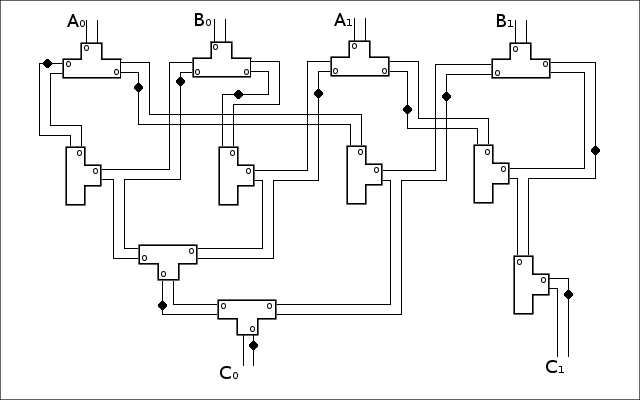
\includegraphics[width=15cm]{bilder/UndGatter.png}
\end{center}    

\subsection{Initialisierung}

\subsection{Korrektheit}



% ----------------------------------------------------------------------------
\section{Zusammenfassung und Ausblick}


\subsection{Geschwindigkeit der Berechnung}

\subsubsection{Ein langes Kabel vs. viele T-Elemente}

\subsection{Implementierung}




\label{sec:summary}

Zum Abschluss kommt das Literaturverzeichnis.
%
Die beiden Zeilen

\begin{tcblisting}{listing only}
  \bibliographystyle{plain}
  \bibliography{\jobname}
\end{tcblisting}

erzeugen das, was man unter dieser Zeile sieht:

\bibliographystyle{plain}
\bibliography{\jobname}

\end{document}
